\documentclass[10pt,letterpaper]{article}
\usepackage[T1]{fontenc}\usepackage[utf8]{inputenc}\usepackage{mathptmx}
\usepackage[margin=0.72in]{geometry}\usepackage{microtype}\usepackage{amsmath}
\usepackage{booktabs}\usepackage{graphicx}\usepackage{caption}\usepackage{tabularx}\usepackage{ragged2e}
\usepackage[hidelinks]{hyperref}
\captionsetup{font=small,labelfont=bf,justification=RaggedRight,singlelinecheck=false}
\newcolumntype{Y}{>{\RaggedRight\arraybackslash}X}
\setlength{\parindent}{0pt}\setlength{\parskip}{4pt}
\title{\vspace{-18pt}\large The ANNNI phase diagram under two classes of error:\\ what depolarizing noise and coherent drift each do to a phase boundary, and what recovers it}
\author{\normalsize Matthew Stanley Leibel, TrueLoop Compute (NEOTECH Inc.) \quad QSITE 2026 Quantum Coalition, Scientific Track}
\date{\normalsize September 2026}
\begin{document}\maketitle\vspace{-16pt}

\textbf{Summary.} We map the phase diagram of the 1D ANNNI model on $N=8$ qubits with a variational circuit that reaches the exact ground state at every grid point, reproduce the ferromagnetic, antiphase, and paramagnetic regions with boundaries on the analytic lines, and then study how errors distort those boundaries. The track's depolarizing noise turns out to be \emph{amplitude loss}: the order-parameter signal shrinks almost uniformly, so a fixed threshold loses every ordered point at $p=0.01$, while an observable rescaled by a reference point recovers 99\% of the classification. Coherent calibration drift, the error class the handout omits but every processor has, is \emph{shape distortion}: it moves the boundary, in a direction set by the sign of the miscalibration, and rescaling cannot touch it. An in-band maintenance layer holding the circuit's angles from five probe circuits per cycle removes 60 to 83\% of the drift-induced boundary shift, keeps the diagram stable over ten unsupervised passes and a calibration jump, and under both errors at once returns the diagram to its depolarizing-only form. The two mitigations are complementary, and together they separate what calibration can recover from what decoherence costs.

\section*{1. Method}
\textbf{Model and observable.} $H=-\sum_i Z_iZ_{i+1}+\kappa\sum_i Z_iZ_{i+2}-h\sum_i X_i$, periodic, on a $15\times15$ grid in $\kappa\in[0,1]$, $h\in[0.05,2]$. The order parameter is the next-nearest correlator $C_2=\tfrac1N\sum_i\langle Z_iZ_{i+2}\rangle$: $+1$ in the ferromagnet, $-1$ in the antiphase ($\uparrow\uparrow\downarrow\downarrow$), small in the paramagnet. It is symmetry-safe at finite size, whereas single-site magnetization and products of single-bond expectations vanish on the symmetric ground state. Thresholds are fixed once on the clean diagram at the analytic Ising and Kosterlitz--Thouless lines ($C_2>0.56$ ferro, $C_2<-0.83$ antiphase) and reused unchanged for every noisy arm. The $\kappa=0.5$ column, where both ordered phases meet at $h=0$, carries no ordered reference and is excluded from rescaled boundaries.

\textbf{Preparation.} A Hamiltonian-variational circuit from $|+\rangle^{\otimes N}$: four layers of $e^{-ig_1\sum ZZ_{nn}}e^{-ig_2\sum ZZ_{nnn}}e^{-ib\sum X}$, 12 parameters, each $RZZ$ compiled as CNOT--RZ--CNOT (128 CNOTs). Optimized by L-BFGS with adjoint gradients, warm-started down the field from the paramagnet where the circuit is exact. Median relative energy error $4\times10^{-5}$, worst $2\times10^{-2}$; $C_2$ within 0.05 of exact diagonalization at 95\% of points. The one outlier, $(0.57, 0.19)$, sits exactly on the analytic KT line, where the exact ground state has $C_2=-0.32$ while three states within 0.063 of it have $C_2\approx-0.95$; the variational state, 0.049 above the ground energy, lands in that manifold. That is a finite-size boundary degeneracy, not an optimizer failure, and we keep the lower-energy state. The live PennyLane optimization in the notebook reaches $1.7\times10^{-5}$ relative error at $(0.3,0.6)$ in 107 evaluations.

\textbf{Two error classes.} Depolarizing: \texttt{DepolarizingChannel}$(p)$ on the target after every CNOT, the starter kit's convention, on PennyLane's \texttt{default.mixed}, $p=0.01$ and $0.05$, all 225 points. Coherent drift: every $RX$ angle scaled by $1+\epsilon_i$ and every $RZZ$ angle by $1+\delta_k$, with $\epsilon,\delta$ drifting across the scan as a static offset plus a mean-reverting wander, half common-mode and half independent, RMS 3\% and 6\%. A numpy density-matrix simulator accelerates the drift study and agrees with \texttt{default.mixed} on the full grid to $2\times10^{-12}$.

\textbf{Maintenance.} Each cycle (one grid point) runs five probe circuits beside the workload: a three-fold amplified rotation on all qubits in one circuit and amplified $RZZ$ probes on the 16 pairs in four, 4,000 shots each. A per-channel controller (TrueLoop v3.1.0, evaluation build shipped with the notebook) holds the 24 channels: it corrects only when a channel's retained residual clears the measured noise floor, learns each slope and sign from the loop's own motion, and applies corrections as multiplicative scales on the next cycle's angles. Nothing is re-optimized; the drift trajectory is identical for the free-running and maintained arms.

\begin{figure}[t]\centering
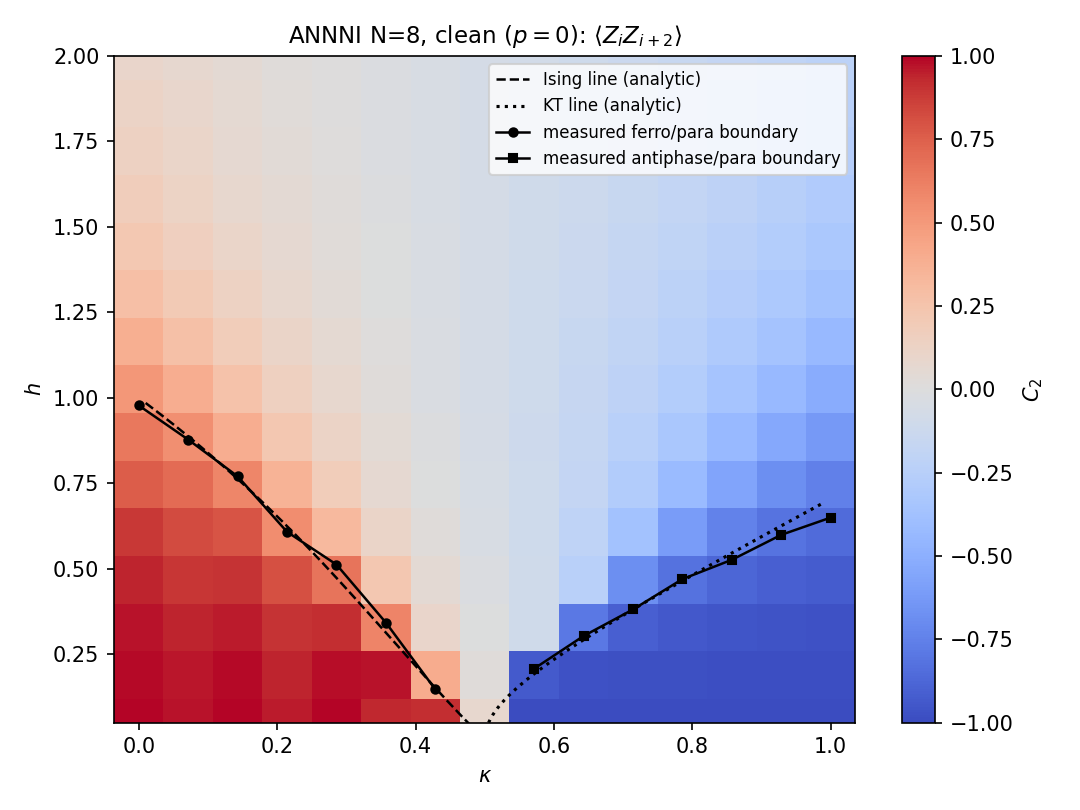
\includegraphics[width=0.44\textwidth]{../figures/phase_diagram_p0.png}\hfill
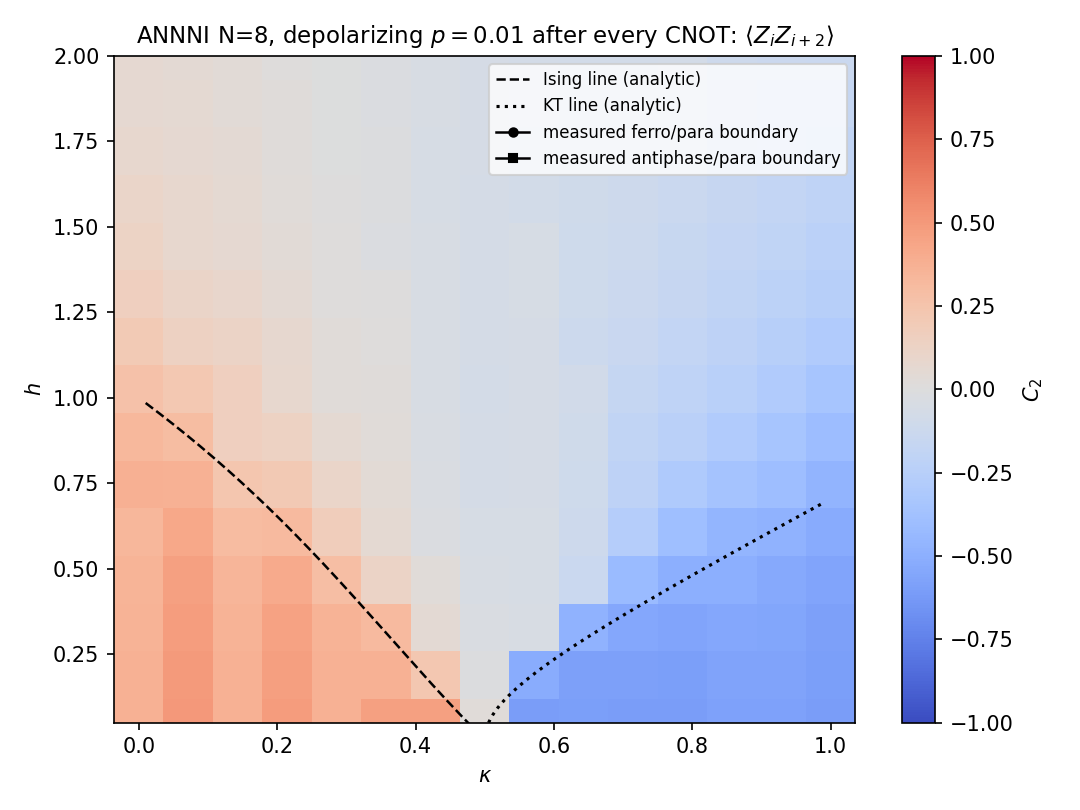
\includegraphics[width=0.44\textwidth]{../figures/phase_diagram_p0.01.png}
\caption{Left: clean diagram, measured boundaries (markers) against the analytic Ising (dashed) and KT (dotted) lines. Right: $p=0.01$ depolarizing after every CNOT. The colour scale is the same; the ordered phases have faded, not moved.}
\end{figure}

\section*{2. Results}
\textbf{Clean diagram.} All three phases appear where they should. The ferro/para boundary at $\kappa=0.29$ is at $h^*=0.512$ against the Ising line's 0.473; the antiphase/para boundary at $\kappa=0.71$ is at $h^*=0.381$, on the KT line's 0.381 (Fig.~1, left).

\textbf{Depolarizing is amplitude loss.} At $p=0.01$ the deep-ordered signal halves (mean $|C_2|$ at $h=0.05$: 0.923 $\to$ 0.483) and at $p=0.05$ it is 5\% of clean (0.049). With the clean thresholds, both noisy diagrams lose every ordered point (24.9\% misclassified). The loss is nearly uniform in $h$, so dividing each column by its value at $h=0.05$, the standard measure-the-decay mitigation, recovers the boundaries at $p=0.01$: misclassification 1.3\%, ferro/para boundary $0.504\to0.559$ at $\kappa=0.29$, antiphase/para $0.381\to0.388$ at $\kappa=0.71$. The residual outward bias comes from the deep-ordered cat-like states being more entangled and losing more than states near the boundary. At $p=0.05$ nothing recovers the diagram. Because the circuit has 128 CNOTs, $p=0.01$ is already 2.6 expected errors per circuit; the relevant parameter is $p$ times depth, not $p$ alone, and an eight-layer circuit (256 CNOTs, exact to three decimals) loses the ordered phases at $p=0.01$ outright.

\textbf{Which phase is most robust.} The antiphase: at $p=0.01$ its deep correlator survives at 0.60 of clean, the ferromagnet's at 0.37. Both finite-size ground states are cat-like superpositions of their classical patterns, but the ferromagnet is prepared with more net $X$ rotation from the paramagnet, so more of its correlation is built late in the circuit after the CNOTs that carry the noise. This is as much a statement about the preparation circuit as about the Hamiltonian, and it reverses the naive expectation that the phase needing two-site correlations is the fragile one. The paramagnet is trivially robust. Under coherent drift the ranking differs: the ferromagnetic boundary moves three times more than the antiphase boundary (0.110 vs 0.033 at 6\%) because $C_2$ is steeper in $h$ there.

\textbf{Coherent drift is shape distortion.} A common 10\% over-rotation moves $C_2$ by $-0.056$ and an under-rotation moves it the other way; across a drifting scan this compounds on the steep parts of the diagram. At 6\% drift the free-running boundary shifts by 0.075 on average, with one excursion of 0.58 at $\kappa=0.14$, and 4.4\% of points are misclassified; rescaling does not reduce it (Table~1).

\begin{table}[h]\caption{Rescaled boundaries, $N=8$, thresholds fixed from the clean diagram. Shifts are mean $|{\Delta h^*}|$ over columns.}
\small\begin{tabularx}{\textwidth}{Y r r r r}\toprule
Arm & misclassified & mean $|\Delta h^*|$ & ferro/para $h^*$, $\kappa{=}0.29$ & antiphase/para $h^*$, $\kappa{=}0.71$\\\midrule
clean & 0.0\% & 0 & 0.504 & 0.381\\
depolarizing $p=0.01$ & 1.3\% & 0.035 & 0.559 & 0.388\\
depolarizing $p=0.05$ & 24.9\% & no boundary & none & none\\
drift 3\%, free-running & 1.3\% & 0.016 & 0.507 & 0.378\\
drift 3\%, maintained & 0.0\% & 0.007 & 0.506 & 0.383\\
drift 6\%, free-running & 4.4\% & 0.075 & 0.515 & 0.374\\
drift 6\%, calibrate once then free-run & 1.3\% & 0.037 & 0.510 & 0.369\\
drift 6\%, maintained (5 circuits/cycle) & 1.8\% & 0.015 & 0.508 & 0.390\\
drift 6\% $+$ $p=0.01$, free / maintained & 3.6\% / 0.4\% off depol-only & 0.070 / 0.038 & 0.574 / 0.562 & 0.383 / 0.399\\
\bottomrule\end{tabularx}\end{table}

\textbf{Maintenance recovers the boundary, and isolates the incoherent part.} Holding the 24 angle channels in-band cuts the mean boundary shift from 0.016 to 0.007 at 3\% drift (55\% removed) and from 0.075 to 0.015 at 6\% (80\%), with the residual angle error at 0.4 of free-running, a floor set by the wander's per-cycle step rather than by shots. Calibrating once at the start of the scan removes only the static half (0.037). Re-optimizing the VQE at every point absorbs the drift completely on an $8\times8$ sub-grid, and so does maintenance, but re-optimization cost 726 evaluations per point, about 36,000 circuits with parameter shift, against five probe circuits per cycle. Under 6\% drift plus $p=0.01$, the maintained diagram differs from the depolarizing-only diagram at 0.4\% of points against 3.6\% free-running, and its boundaries land on the depolarizing-only ones (0.562 against 0.559): maintenance returns the diagram to its incoherent-only form.

\textbf{Continuous operation.} Ten consecutive passes at 6\% drift, 2,250 cycles, with every static offset redrawn at pass 5 and nobody intervening: residual 0.062 $\to$ 0.024 in every pass, misclassification 3--4\% $\to$ 0--2\%, pass-to-pass boundary standard deviation 0.051 $\to$ 0.020, the jump absorbed in three cycles, host time 47\,$\mu$s per cycle. At $N=12$ with 36 channels the ratio is the same (0.062 $\to$ 0.025), stability 0.025 $\to$ 0.007, host 76\,$\mu$s per cycle.

\textbf{Complexity decoupled from the state.} Two things keep continuous hardware in a laboratory. A person has to recalibrate it on a schedule, so it cannot run unsupervised and cannot follow a wander faster than the schedule; or the host has to reconstruct the device's state to correct it, which costs $n^2$ memory and $n^3$ setup and cannot reach high dimension. The contract does neither: it holds $3N$ channels from one parallel read, while the state it protects has $2^N$ amplitudes. The continuous scan of the $\kappa=0.29$ column was repeated at $N=8,12,16,20$ with eight-layer circuits (exact to $10^{-3}$ at $N=12$, within 0.14 in the ordered phase at $N=16$, and at $N=20$ carrying the $N=16$ angles), on one drift trajectory, with a third arm in which an engineer recalibrates every 50 cycles (Table~2). From $N=8$ to $N=20$ the state dimension grows 4,096-fold and the classical cost of merely evaluating the state 8,800-fold, from 1\,ms to 5.2\,s; the host's maintenance cost grows 2.8-fold, linear in channels at 2.6\,$\mu$s each. At every size the contract holds the boundary tighter than the scheduled engineer, and at $N=12$ it holds it three times tighter. The correction bounds were set to $[0.85,1.15]$ so that bounds times drift stays inside the three-fold probe's monotone range; with wider bounds one channel at $N=16$ left that range, learned an inverted slope and ran to its bound, which is the capture-range rule stated in the notebook.

\begin{table}[h]\caption{Decoupling: continuous scans at fixed $\kappa=0.29$, 6\% drift. Angle error RMS over the run and mean $|\Delta h^*|$ against the clean circuit; ``eng'' recalibrates every 50 cycles.}
\small\begin{tabularx}{\textwidth}{r r r r r r Y Y}\toprule
$N$ & state dim & channels & cycles & host $\mu$s/cycle & state eval & angle error free / eng / contract & boundary shift free / eng / contract\\\midrule
8 & 256 & 24 & 150 & 56 & 1\,ms & 0.061 / 0.051 / 0.046 & 0.014 / 0.006 / 0.007\\
12 & 4,096 & 36 & 150 & 85 & 9\,ms & 0.051 / 0.047 / 0.028 & 0.085 / 0.064 / 0.025\\
16 & 65,536 & 48 & 144 & 129 & 242\,ms & 0.059 / 0.046 / 0.031 & 0.018 / 0.016 / 0.008\\
20 & 1,048,576 & 60 & 18 & 159 & 5.2\,s & 0.043 / -- / 0.029 & 0.023 / -- / 0.015\\
\bottomrule\end{tabularx}\end{table}

\section*{3. Interpretation and limitations}
In the language of the model, depolarizing shortens every correlation length uniformly, so order parameters shrink without the boundaries moving, and a ratio observable sees the boundary until the correlation length falls below two sites. Coherent drift changes the effective Hamiltonian the circuit prepares, shifting where frustration and field balance; that is a real boundary shift. Rescaling fixes the first, maintenance fixes the second, and neither substitutes for the other. The floating phase is not resolved: at $N=8$ it cannot be separated from the antiphase boundary region, and the two poorly converged points near $\kappa\approx0.6$ sit exactly there. Limitations: $N=8$ periodic for the full diagram; noise after CNOTs only; a drift model whose wander speed sets the residual; and one product boundary found on the way: with link signs declared and a 4,000-shot probe under 6\% drift, the controller's one-time slope identification mis-read up to ten channels and held them (never worse than free-running, but unmaintained); letting its preflight learn the signs removed the failure, and that is the configuration used. Code, cached data, and the executed notebook reproduce every number here.

\vspace{2pt}\scriptsize\textbf{References.} [1] Quantum Coalition, \emph{QSITE 2026 Scientific Track handout and starter kit}, github.com/benmcdonough20/QSITE-2026-QuantumCoalition (Hamiltonian builder, observables, analytic lines). [2] PennyLane demo ``ANNNI Phase Detection'' (pennylane.ai/qml/demos/tutorial\_annni): the Ising and Kosterlitz--Thouless boundary formulas used as reference lines. [3] PennyLane challenge ``A Noisy Heisenberg Model'' (pennylane.ai/challenges/heisenberg\_model): the depolarizing-after-every-CNOT convention. [4] V.~Bergholm et al., ``PennyLane: Automatic differentiation of hybrid quantum-classical computations,'' arXiv:1811.04968 (2018); PennyLane 0.45.1 used. [5] W.~Selke, ``The ANNNI model: theoretical analysis and experimental application,'' Phys.\ Rep.\ 170, 213 (1988). [6] M.~S.~Leibel, ``A Stability Contract for Scalable Hybrid Computing: Minimal Sufficient Control of Component-Observable Hardware,'' Preprints 202609.1101 (2026), doi:10.20944/preprints202609.1101.v1, under review at IEEE Trans.\ Computers: the maintenance layer's method and bounds; the evaluation build of TrueLoop v3.1.0 (NEOTECH Inc.) is included. [7] NumPy, SciPy, Matplotlib.

\end{document}
